\chapter{Аналитический раздел}
В данном разделе рассматриваются сферы применения методов распознавания действий человека, описываются 
алгоритмы детектирования объектов с помощью дескрипторов, алгоритмы классификаторов, их достоинства и недостатки.
Проводится классификация уже существующих методов распознавания действий человека, представлены результаты сравнения рассмотренных методов. Описываются требования к набору данных для обучения модели и его структура.

\section{Обзор областей применения методов распознавания физической активности человека}

Распознавание видов физической активности человека является одной из актуальных задач в области машинного обучения из-за сложности и разнообразия видов физической активности, выполняемых человеком.

Целью распознавания является определение деятельности человека на основе данных датчиков для последующего анализа системой с учетом практической задачи.

Сложный и изменчивый характер данных об активности создает многочисленные проблемы, которые влияют на производительность систем, используемых для решения
практических задач. Ниже рассмотрим некоторые области применения технологии распознавания физической активности человека.


\subsection{Безопасность}

Системы видеонаблюдения являются одним из основных средств обеспечения
безопасности на объекте информатизации. Видео с дорожных и уличных камер могут содержать как моменты рядовых событий, так и моменты правонарушений, которые требуют своевременной фиксации и передачи в правоохранительные органы. Автоматическая идентификация, при помощи камер
наружного наблюдения, преступников и террористов по характерным
жестам, позволит существенно упростить работу правоохранительных органов и, потенциально, спасти множество жизней. 
\clearpage
Задача автоматизации процесса анализа видеопотока с целью выявления инцидентов, возникающих на контролируемом объекте. В настоящее время уже существует множество разработок, направленных на предварительный анализ происходящего на видеоизображении: забытые предметы, оружие, проход людей в запретную зону (например, выход на железнодорожные пути), драки и т.п. 

В статье \cite{safe} предложено применение подхода переноса знаний для распознавания агрессии на видеоизображении с использованием трех моделей трехмерных сверточных искусственных нейронных сетей (ИНС) в качестве экстрактора признаков.

\subsection{Медицина}

В области медицины приложения для распознавания физической активности также
играют важную роль, так как позволяют дистанционно контролировать корректность выполнения рекомендаций или плана, назначенного врачом, тем самым сокращая время пребывания пациента в больнице.

После перенесенной болезни пациенту необходимо пройти реабилитацию. Физическая телереабилитация подразумевает дистанционный мониторинг выполнения пациентом физических упражнений с целью восстановления здоровья, физического состояния и его трудоспособности.


\subsection{Производство и образование}

Факт нахождения человека на рабочем месте не подразумевает того, что работник
эффективно выполняет свои обязанности. Распознавание видов активности в сфере производства и услуг позволит контролировать эффективности работы сотрудников, выявлять нелояльных сотрудников, некачественное выполнение работы и мошеннические
схемы. На основе полученных данных руководители организаций и предприятий смогут своевременно принимать меры по оптимизации работы персонала и повысить эффективность производственных процессов.

Высокие технологии глубоко проникли в сферу образования. Системы видеонаблюдения существуют во всех учебных заведениях.

В статье \cite{ex} описан метод распознавания действий учащихся на видеопоследовательности с экзамена.\newline Аномальными ситуациями в данном
случае понимаются нарушения правил проведения экзамена: списывание, использование запрещенных предметов, нарушения со стороны организаторов экзамена.

\section{Алгоритмы классификации}
Для решения задачи распознавания действий необходимо рассмотреть алгоритмы классификации. Алгоритмы решают задачу  распределение объектов по группам (классам) на основании каких-либо признаков. Класс -- это множество объектов, имеющих определенный общий признак, отличающий эту совокупность от других объектов. Рассмотрим следующие
методы классификации: метод Байеса, деревья решений, метод k-ближайших соседей, метод опорных
векторов, случайный лес.

\subsection{Метод Байеса}

Метод относится к
вероятностным методам классификации. Для каждого наблюдения их множества $X$
высчитывается вероятность его возникновения
в соответствующем классе по формуле:


\begin{equation}
	P(x_{i}|y_{i}) = \frac{count(x_{i}|y_{i})}{count(X|y_{i})},
\end{equation}

где $count(x_{i}|y_{i})$ -- количество элементов $x_{i}$ в
категории $y_{i}$. $count(X|y_{i})$ -- количество наблюдений из множества $X$ принадлежащих категории $y_{i}$.
Для того что бы учитывать категории с небольшим количеством наблюдений используется нормализация. Тогда вероятность вычисляется по формуле:

\begin{equation}
	P(x_{i}|y_{i}) = \frac{\frac{count(x_{i}|y_{i})}{count(X(y_{i})}}{\sum\limits_{j}^{n}\frac{count(x_{i}|y_{n})}{count(X|y_{n})} },
\end{equation}

При вычислении вероятности по формуле (1.3) требуется так
же априорная вероятность возникновения категории $y_{i}$ равна отношению числа наблюдений
в  $y_{i}$ к общему числу наблюдений.

\begin{equation}
	P(x_{i}|y_{i}) = \frac{count(X|(y_{i})}{count(X)},
\end{equation}

где $count(X|(y_{i})$ -- число наблюдений принадлежащих категории $y_{i}$, $count(X)$ -- общее
число наблюдений.

Классификация набора наблюдений
происходит после вычисления вероятности по
формуле:

\begin{equation}
	P(X|y_{i}) = P(y_{i})\prod\limits_{j}^{n}p(x_{j}|(y_{i})),
\end{equation}

где $P(y_{i})$ -- априорная вероятность возникновения $y_{i}$, $p(x_{j}|y_{i})$ -- вероятность возникновения наблюдения $x_{j}$ в категории $y_{i}$ \cite{baes1}.

%(все выше эта статья http://www.vestnik.vsu.ru/pdf/analiz/2009/02/2009-02-05.pdf)

В статье \cite{baes2} перечислены достоинства и недостатки метода Байеса.

Преимущества метода:
\begin{itemize}
	\item[---] высокая скорость работы;
	\item[---] относительно простая программная
	реализация алгоритма;
	\item[---] легкая интерпретируемость результатов
	работы алгоритма.
\end{itemize}

Недостатки метода: относительно низкое качество классификации и неспособность учитывать
зависимость результата классификации от сочетания признаков.

%(достоинстав отсюда https://cyberleninka.ru/article/n/metody-avtomaticheskoy-klassifikatsii-tekstov/viewer)

%Пусть $P(ci|d)$ – вероятность того, что документ,
%представленный вектором $d = (t1, …, tn)$, соответствует категории $c_{i}$ для $i = 1, …, |C|$. Задача классификатора заключается в том, чтобы подобрать такие значения $c_{i}$ и $d$, при которых значение вероятности $P(c_{i}|d)$ будет максимальным:

%\begin{equation}
%	CSV(d) = arg max P(c_{i}|d)
%\end{equation}
%,где $c_{i} \in$ С.

%Для вычисления значений $P(c_{i}|d)$ пользуются
%теоремой Байеса:

%\begin{equation}
%	P(c_{i}|d) = \frac{P(c_{i})P(d|c_{i})}{P(d)},
%\end{equation}

%где  $P(ci)$ -- априорная вероятность того, что документ отнесен к категории $c_{i}$;  $P(c_{i}|d)$ -- вероятность

\subsection{Метод опорных векторов}

Метод опорных векторов является широко распространенным методом, который используется в методах оптимизации, а также и в машинном обучении.

Суть задачи классификации заключается в построении алгоритма классификации по обучаемой выборке. Идея линейных классификаторов заключается в
построении линейных функций, являющимися разделяющими поверхности, по
обе стороны которой лежат объекты разных классов. При использовании метода
опорных векторов используется функционал особого вида:

\begin{equation}
	\sum\limits_{i=1}^{l}(1-M_{i}(w,w_{0})) + \frac{1}{2C}\|w\|^2 \rightarrow min_{w,w_{0}},
\end{equation}
где $M_i(w,w_0) = y_i((w, x_i) - w_0)$ -- величина отступа.

Пусть имеем объекты, принадлежащие двум классам. Если выборка является линейно разделимой, то оптимальную разделяющую поверхность можно
найти из решения системы:


\begin{equation}
	\begin{cases}
		\|w\|^2 \rightarrow min,\\
		M_i(w,w_0) \geq 1, i = 1, .., l. \\
	\end{cases}
\end{equation}

C учетом того, что выборка на практике чаще всего не является линейно
разделимой, ограничение в системе становится менее жестким:

\begin{equation}
	\begin{cases}
		\frac{1}{2}\|w\|^2 + C 	\sum\limits_{i=1}^{l} \xi_{i}\rightarrow min_{w,w_{0},\xi},\\
		M_i(w,w_0) \geq 1 - \xi_{i}, i = 1, .., l\,\
		\xi_{i} \geq 0, i = 1, .., l. \\
	\end{cases}
\end{equation}

При решении системы в зависимости от параметров получаются 3 типа объектов \cite{vec}:

\begin{itemize}
	\item[---] периферийные, неинформативные объекты;
	\item[---] опорные;
	\item[---] объекты, которые оказались по другую сторону от разделяющей поверхности.
	
\end{itemize}

В статье \cite{baes2} перечислены достоинства и недостатки метода опорных векторов.

Достоинства: за счет применения гиперплоскостей работает при малых объемах обучающей выборки. За счет использования ядра
описывающего связь между элементами выборки, можно использовать гиперплоскости разной
сложности.

Недостатки: большое время обучение, необходимость ядра для конкретного случая.

\subsection{Метод k-ближайших соседей}

Метод ближайших соседей -- один из самых простых классификаторов,
основанный на оценивании сходства признаков объектов. Классифицируемый
объект относится к тому классу, к которому принадлежат ближайшие к нему
объекты обучающей выборки. Первоначально задаем обучающую выборку пар «объект-класс»: 

\begin{equation}
	X^m = {(x_{1}, y_{1}), ..., (x_{m}, y_{m})}.
\end{equation}

%Это могут быть объекты, которые ранее уже были классифицированы,
%либо объекты, которые классифицируют эксперты. Теперь на множестве
%объектов зададим метрику $p(x,x^'$): она обратно пропорциональна сходству
%между объектами $x,x^'$. 

Для произвольного объекта $u$ расположим объекты обучающей выборки
$x_{i}$ в порядке возрастания расстояния до $u$:

\begin{equation}
	p(u,x_{1;u}) \leq p(u,x_{2;u}) \leq ... \leq p(u,x_{m;u}),
\end{equation}

где через $x_{1;u}$ обозначается тот объект обучающей выборки, который
является $i$ соседом объекта $u$. Так же перенумеруем классы, к которым
относятся  $x_{1;u}$ -- обозначим их  $y_{i;u}$. Алгоритм ближайших соседей в общем виде можно выразить формулой:

\begin{equation}
	a(u) = arg max \sum\limits_{i=1}^{m}[y(x_{1;u}) = y]w(i,u).
\end{equation}

Здесь $w$ весовая функция, показывающая, важен ли для объекта элемент
под номером i. Для метода k ближайших соседей $w(i,u) = [i \leq k]$. Таким
образом, алгоритм классификации методом ближайших k соседей очень
прост. У нас есть выборка из данных -- обучающее множество, для каждого
элемента которого известно, к какому классу он принадлежит.
Для каждого следующего элемента неизвестного класса берется выборка
из k ближайших элементов, класс которых уже известен. Новому элементу
присваивается тот класс, элементов которого оказалось больше всего в
выборке \cite{ksosed}.

В статье \cite{baes2} перечислены достоинства и недостатки метода k-ближайших соседей.

Преимущества метода:
\begin{itemize}
	\item[---] возможность обновления обучающей выборки без переобучения классификатора;
	\item[---] устойчивость алгоритма к аномальным выбросам в исходных данных;
	\item[---] хорошее обучение в случае с линейно неразделимыми выборками.	
\end{itemize}

Недостатки метода:
\begin{itemize}
	\item[---] репрезентативность набора данных, используемого для алгоритма;
	\item[---] высокая зависимость результатов классификации от выбранной метрики;
	\item[---] большая длительность работы из-за необходимости полного перебора обучающей выборки;
	\item[---] невозможность решения задач большой размерности по количеству классов и документов.

\end{itemize}

\subsection{Деревья решений}

Классификация является одной из задач, где используются деревья
принятия решений. Они создают иерархическую структуру классифицирующих правил типа «если…то», имеющую вид дерева. Для принятия решения, к какому классу отнести некоторый объект или ситуацию, требуется ответить на вопросы, стоящий в узлах этого дерева, начиная с его корня. Основа такой структуры -- ответы «Да» или «Нет» на ряд вопросов.

Рассмотрим два наиболее известных алгоритма построения деревьев решений CART и C4.5 для задачи классификации. Основным отличием данных алгоритмов является устойчивость к шумам и выбросам данных. Алгоритм CART решает задачи классификации и является самым распространенным способом выявления, структурирование и графического представления логических закономерностей в данных. Его преимущество заключается в следующем \cite{tree2}:
\begin{itemize}
	\item[---] быстрый процесс обнаружения знаний;
	\item[---] генерация правил в предметных областях, в которых трудно  формализуются знания;
	\item[---] извлечение правил на естественном языке;
	\item[---] создание интуитивно понятной классификационной модели предметной области;
	\item[---] прогноз с высокой точностью, сопоставимой с другими методами;
	\item[---] построение непараметрических моделей.
\end{itemize}
В данном алгоритме можно выделить три основные операции: сортировка источника данных при формировании множества условий для атрибутов числового типа, вычисление критерия Gini при разбиении узлов бинарного дерева, перемещение в таблице значительных объемов информации при деление узла.

Отбор наилучшего варианта разбиения узла дерева проводится наибольшей классифицирующей силе, вычисляемой по критерию Gini:
\begin{equation}
	GINI =  \frac{1}{|L|}\sum\limits_{i=1}^{Ncp}(l_{i})^2 + \frac{1}{|R|}\sum\limits_{i=1}^{Ncp}(r_{i})^2.
\end{equation}

Алгоритм C4.5 строит дерево решений с неограниченным количеством ветвей у узла. Данный алгоритм может работать только с дискретным зависимым атрибутом и поэтому может решать только задачи классификации.
Его преимущества заключаются в следующем \cite{tree2}:
\begin{itemize}
	\item[---]  C4.5 использует относительную энтропию при генерировании деревьев решений;
	\item[---] C4.5 использует однопроходное отсечение ветвей, чтобы упростить переобучение. Это сущетсвенно улучшает работу алгоритма;
	\item[---]  C4.5 может работать  и с непрерывными и с дискретными данными.
\end{itemize}



В статье \cite{baes2} перечислены достоинства и недостатки метода деревья решений.

Преимущества метода:
\begin{itemize}
	\item[---] высокая скорость работы;
	\item[---] относительно простая программная
	реализация алгоритма.
\end{itemize}

Недостатки метода: неустойчивость алгоритма по отношению к выбросам в исходных данных и большой объем данных для получения точных результатов.

\subsection{Метод случайного леса}

Метод случайного леса
основан на построение так называемого
ансамбля деревьев решений. Алгоритм
получился сложением двух основных
идей: метод бэггинга и метод случайных подпространств. Данный метод
используется для решения задач классификации, регрессии и кластеризации.


Деревом решений обычно называют
представление правил в иерархической,
последовательной структуре, где каждому объекту соответствует узел, дающий решение. Под правилом понимается логическая структура «если…то». 


Удобство применения построения
дерева решений состоит в удобном представлении знаний в экспертных системах, а именно после написания совокупности правил их легко можно изобразить
в виде графа, это и удобно, и более
наглядно, чем перечисление правил.
Пусть имеется некоторая выборка
из $m$ на $n$ элементов.

Можно произвольно взять некоторые данные из этой выборки и на ее
основе построить дерево решений, пример построения дерева приведен на рисунке 1.1. Таким же образом проделать и с другими данными. Вся особенность это
алгоритма состоит в универсальности,
быстроте и случайности построения
деревьев решений. Дерево строится без
отсечения ветвей (как это можно увидеть при построении деревьев алгоритмов типа CART или С4.5, \newline 
т.е. происходит
построение полных деревьев).

\begin{figure}[h]
	\begin{center}
		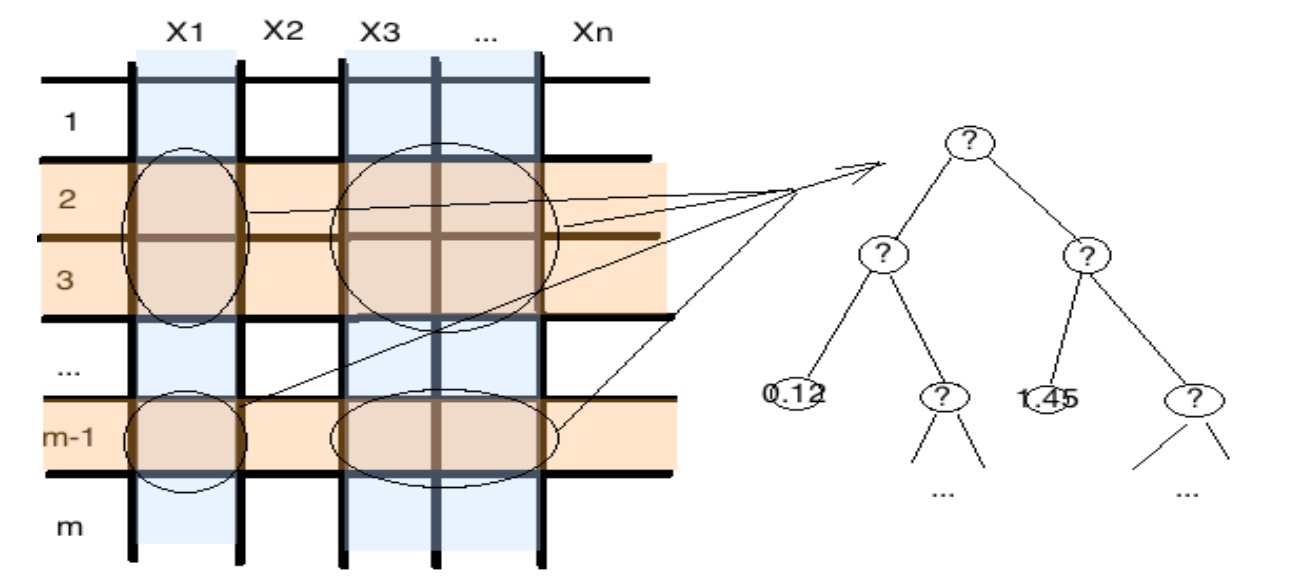
\includegraphics[ scale=0.37]{./img/randomtree.jpg}
		\caption{Выбор случайных данных и построение на их основе дерева решений}  
		\label{fig:xray1}
	\end{center}
\end{figure}

Далее результат будет либо усредняться (в случаи регрессии) или путем
голосования (в случае классификации).
На каждом шаге построения дерева
решения нужно выбирать признак и
значение порога, который будет соответствовать наилучшему результату по
некоторому заданному критерию. Для
решения прикладных задач используют
критерий Джини.

Существуют ряд преимуществ данного метода \cite{randomForest}:
\begin{itemize}
	\item[---] имеется встроенная проверка качества;
	\item[---] повышение точности;
	\item[---] простота применения, т.к. основными параметрами является количество деревьев в ансамбле и количество
	признаков, по которым эти деревья будут расщепляться;
	\item[---] обработка данных с большим количеством признаков и классов;
	\item[---] высокая параллелизуемость.
\end{itemize}

Помимо отмеченных достоинств также существует и недостатки применения:
\begin{itemize}
	\item[---] 	высокая алгоритмическая сложность;
	\item[---] большое количество получившихся деревьев.
\end{itemize}

%( про случайные леса все отсюда https://elibrary.ru/download/elibrary_28087207_40532052.pdf)

\subsection*{Выводы}
 Для реализации метода распознания спортивных действий на видео был выбран алгоритм случайного леса, поскольку он хорошо справляется с большими наборами данных, алгоритм легко распараллелить при программной реализации, устойчив к выбросам, после обучения модели можно определить какая из функций была важнее, а также алгоритм применим в сочетание с методом градиентного бустинга.
%\subsection{Сравнение методов классификаторов}
%Достоинства и недостатки выше описанных методов, указанные в работе \cite{table}, представлены в таблице 1.1.

%\begin{table}[pt!] 
%	\begin{center}
%		\caption{Сравнение методов классификаторов}
%		\label{cmptable}
%		\begin{tabular}{| p{3cm} | p{6cm} | p{6cm} |}
%			\hline
%			\textbf{Метод} 	& \textbf{Достоинства} & \textbf{Недостатки} \\
%			\hline
%			С4.5 			& Простая реализация, интерпретация и отсутствие подготовки данных для их дальнейшего использования. Работа с категориальными и интервальными переменными. Использование модели «белого
%			ящика», её оценка. Работа с большим объёмом информации. & Отсутствие оптимальности дерева
%			решений в целом, необходимость регулировки его длины. Переизбыток
%			данных и плохая читабельность.я\\
%			
%			
%			\hline
%			К-ближних соседей  	& Простота реализации, высокое быстродействие, работа с большим количеством
%			данных.
%			& Наличие неточностей в кластеризации, необходимость начального
%			определения точного числа классов,
%			чувствительность к выбору центров
%			кластеров. \\
%			\hline
%			Метод
%			опорных
%			векторов
%			
%			& Высокое быстродействие, единственно
%			
%			верное решение, нахождение максимальной ширины полосы разделения, вследствие чего производится уверенная классификация. & Большая чувствительность к шумам,
%			
%			стандартизации исходных данных,
%			
%			отсутствие общего подхода к автоматическому выбору ядра в случае
%			
%			линейно неразделимости классов. \\ 	\hline
%			CART 	& Непараметрический метод. Не нужно рассчитывать различные параметры вероятностного распределения. Отсутствие
%			необходимости выбора переменных при
%			анализе данных. Нечувствительность к
%			шумам, высокое быстродействие. & Нестабильность дерева решений.
%			Некорректное отображение деревьев со сложной структурой.
%			\\			
%			\hline
%		\end{tabular}
%	\end{center}
%\end{table}

%Исходя из данной таблицы, для распознавания видов физической активности лучше использовать метод опорных векторов. Метод %опорных векторов позволяет проводить обучение в условиях поступления данных в реальном времени, обеспечивает уверенную %классификацию и работает по
%малой выборке обучающих данных. 


\section{Обзор алгоритмов детектирования объектов с помощью дескрипторов}

При классификации изображений их упрощение происходит засчет извлечения важной информации. Оригинальное изображение содержит слишком много дополнительной информации, которая не требуется для классификации. Этот шаг
называется извлечением объекта. Существуют специальные алгоритмы, решающие эту задачу. Существует довольно большое количество методов, используемых в компьютерном зрении для решения этой задачи, среди них: HOG (гистограмма направленных градиентов), SIFT (масштабно-инвариантное преобразование признаков), SURF (ускоренная надежная функция) и RIFF.

Для рассмотрения перечисленных алгоритмов также необходимо упомянуть понятие дескриптор. Дескриптором (вектором признаков) называется набор численных параметров, описывающих
характеристики объекта (или его части), например цвет, форму и т.д. Векторы признаков принимают значения в пространстве признаков. 

Дескрипторы разделяют на глобальные, описывающие объект целиком, и локальные, описывающие значимые части объекта или изображения. Основной областью применения локальных дескрипторов является анализ изображений при моделировании компьютерного зрения \cite{deck}.  

Ниже рассмотрим упомянутые алгоритмы.

\subsection{Алгоритм SIFT (масштабно-инвариантное преобразование признаков)}

SIFT является одним из наиболее часто используемых алгоритмов описания дескрипторов
особых точек на изображении. Дескрипторы, полученные с помощью этого алгоритма инвариантны к масштабированию и поворотам изображения, устойчивы
к изменениям освещения, шумам и изменениям
позиции наблюдателя \cite{sift1}. 

Характерной особенностью алгоритма SIFT является применяемый в них метод
определения позиций структурных элементов:
ключевые точки (центры локальных регионов,
описываемых SIFT-дескрипторами) выбираются там, где результаты фильтрации изображения с использованием детекторов Харриса
или Гессе имеют экстремумы. 

Анализ
изображения производится последовательно для разных коэффициентов его масштабирования, а содержание локального региона,
описываемого SIFT-дескриптором, нормализуется относительно вращения. Такой способ
описания структурных элементов делает их
инвариантными к смещениям, масштабированию и вращению в плоскости изображения \cite{sift2}.


В статье \cite{siftsurf} выделяются следующие этапы метода SIFT:
\begin{itemize}
	\item[---] определение локальных особенностей (ключевых точек);
	\item[---] локализация особенностей;
	\item[---] вычисление ориентаций особенностей;
	\item[---] описание локальных особенностей через дескриптор;
	\item[---] сопоставление дескрипторов. 	
\end{itemize}



\subsection{Алгоритм SURF (ускоренная надежная функция)}
Метод SURF ищет ключевые точки и строит описание найденных ключевых точек через дескрипторы особенностей и является аналогом метода SIFT. Ключевой точкой является локальный экстремум детерминанта матрицы Гессе. Для двумерного случая
детерминант матрицы Гессе определяется следующим образом:

\begin{equation}
	det(H) =  \frac{\partial^2f}{\partial x^2} \frac{\partial^2f}{\partial y^2} 
	-  (\frac{\partial^2f}{\partial x \partial y})^2,
\end{equation}

где \newline
\hspace*{30mm} матрица Гессе:             

\begin{equation}
	H(f(x,y)) = \begin{pmatrix}
		\frac{\partial^2f}{\partial x^2} & \frac{\partial^2f}{\partial x \partial y} \\
		\frac{\partial^2f}{\partial x \partial y} & \frac{\partial^2f}{\partial y^2}
	\end{pmatrix},	
\end{equation} 
\begin{center}
	$f(x,y)$ -- функция изменения градиента яркости.    
\end{center}


Гессиан инвариантен к сдвигу яркости изображения и повороту, но не инвариантен к масштабу. Данную проблему решают с помощью последовательного
перебора различных масштабов и фильтров и поочередного применения их к
одному пикселю. В качестве опорных точек выбирают локальные максимумы
гессианов, соответствующие локальным максимумам изменения градиента яркости. 

После нахождения точек локальных максимумов определяют точка истинного максимума гессиана. Данная методика гарантирует, что в окрестности ключевой точки расположены участки с разными градиентами. Дескриптор
представляет собой массив чисел, определяющих опорную точку. Инвариантность дескриптора относительно поворота обеспечивается дисперсией (различием) дескрипторов для разных особых точек.

Для определения особых точек в методе SURF используется целочисленная
аппроксимация детерминанта blob-детектора гессиана, который вычисляется с
помощью трех операций с использованием предварительно вычисленного 
интегрального изображения. Blob-детектирование -- выявление областей в
цифровом изображении, которые отличаются по своим свойствам, таким как
яркость или цвет, от прилегающих областей \cite{siftsurf}. 


Также в статье \cite{siftsurf} выделяются следующие этапы алгоритма работы SURF:
\begin{itemize}
	\item[---] масштабно-пространственное представление;
	\item[---] расчет значений гессиана;
	\item[---] поиск точек локальных максимумов;
	\item[---] определение точки истинного максимума;
	\item[---] определение ориентации опорной точки;
	\item[---] формирование дескриптора опорной точки. 	
\end{itemize}



\subsection{Метод RIFF (Rotation Invariant Fast Features)}
В основу метода RIFF положено радиальное
и тангенциальное разложение гистограмм
градиента и последующая обработка по кольцам.
Дескриптор также инвариантен к масштабированию, вращению и изменению освещенности.

Дескрипторы RIFF формируются достаточно быстро для обеспечения отслеживания объектов со скоростью следования кадров или близко к скорости следования кадров и достаточно устойчиво для решения задач крупномасштабного распознавания. Формирование дескриптора RIFF может начинаться с процедуры формирования дескриптора сжатой гистограммы градиентов (CHoG, compressed histogram of gradient) \cite{sift1}.

%\subsection{Вывод}

%В работе \cite{sift1} основным недостатком методов SIFT и
%SURF выделяют нечеткое выделение объекта
%относительно фона и низкий процент правильного распознавания элементов изображений
%объектов без ярко выраженной текстуры.

%Метод RIFF также показал плохие результаты, вызываемые размытием изображения
%вследствие движения наблюдателя с камерой
%относительно неподвижных объектов.
%Поэтому для выделения особых точек и
%идентификации реального объекта в нашем
%случае разработана методика выделения особых точек с использованием рандомных деревьев для подсистемы распознавания в структуре системы проектирования компонент расширенной реальности. 

%вот тут математика для sift и surf (https://elibrary.ru/item.asp?id=41271879)


\subsection{HOG (Гистограмма направленных градиентов)}\label{hog}


Описание объектов составляется из признаков, выбор признаков определяется результативность работа системы. Одним из видов признаков являются признаки формы. Чаще всего при детектирование человека и его движения используются признаки формы и текстуры. Признаки формы описывают расположение и направление переходов на изображении, оценивают градиент. Более простые признаки стремятся найти простые геометрические фигуры на изображении и определить, являются ли наборы этих фигур человеком.

Следующим методом является метод под названием гистограмма направленных градиентов. Данный метод был предложен в далеком 2005 г., это был
один из самых первых алгоритмов, который мог довольно быстро и качественно решать задачу по распознаванию образов на изображениях. Главной идеей
данного алгоритма было то, что любое изображение можно было описать распределением градиентов интенсивности и направления \newline краев \cite{hog1}. 

Алгоритм преобразовывает изображение формата w·h·3 в вектор значений, характеризующихся величинами, получаемых в процессе вычисления вертикальных и горизонтальных градиентов.
Это достигается путем фильтрации изображения с помощью представленных
ядер, показанных на \newline рисунке 1.2.

\begin{figure}[h]
	\begin{center}
		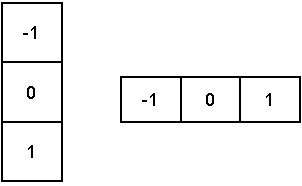
\includegraphics[ scale=1.3]{./img/hog1.pdf}
		\caption{Представление ядер}  
		\label{fig:xray1}
	\end{center}
\end{figure}

%В статье \cite{hog2} автор говорит о том, что гистограмма ориентированных %градиентов (HOG) 

Величина и направление градиентов:

\begin{equation}
	M(magnitude) = \sqrt{G_{x}^2 + G_{y}^2},\\ 	
\end{equation}
\begin{equation}
	D(direction) = \arctan{\frac{G_{x}}{G_{y}}},
\end{equation}

где  
\begin{equation}
	G_{x}= \lim_{\bigtriangleup x\to 1} \frac{f(x_{0}+ \bigtriangleup x) - f(x_{0})}{\bigtriangleup x}= f(x_{0}+ 1) - f(x_{0}),
\end{equation}	
\begin{equation}
	G_{y}= \lim_{\bigtriangleup y\to 1} \frac{f(y_{0}+ \bigtriangleup y) - f(y_{0})}{\bigtriangleup y}= f(y_{0}+ 1) - f(y_{0}).
\end{equation}

Величина градиента показывает, насколько контрастен переход от цвета к
цвету в определенной области. При анализе каждого пикселя изображения на
выходе значение величины -- это максимальная среди всех возможных разностей между значениями цвета \cite{hog1}. 

Обычно их построение происходило путем разбиения изображения на множество ячеек, каждой из которых присваивались гистограммы направлений градиентов для пикселей внутри ячейки. Среднестатистический размер такой ячейки -- 8$\times$8 пикселей. Каждая такая ячейка преобразовывается к
вектору 9$\times$1, в каждой из компонент которого лежит некоторое значение, показывающее порядок величины в определенном направлении, то есть каждый
элемент вектора соответствует градусу -- 0, 20, … , 160 (рассматриваются беззнаковые градиенты), представлена на рисунке 1.3 \cite{hog2}.

\begin{figure}[h]
	\begin{center}
		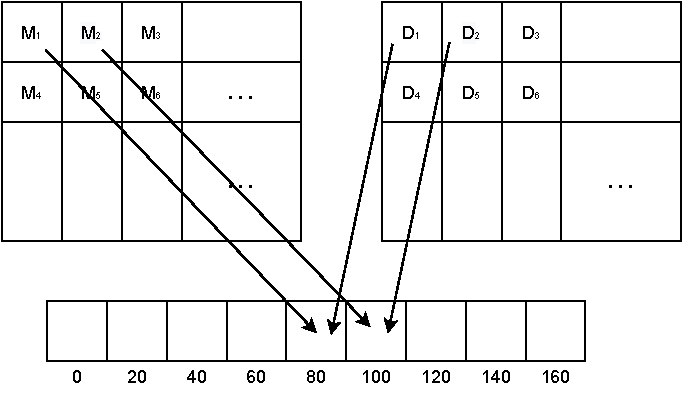
\includegraphics[ scale=1]{./img/hog2.pdf}
		\caption{Гистограмма преобразования}  
		\label{fig:xray1}
	\end{center}
\end{figure}

Для того чтобы получить наилучший и более точный результат, изображение, которое бралось для обработки, приводили к черно-белому
виду, а локальные гистограммы нормализовали по контрасту относительно интенсивности. Нормализация по контрасту является очень важным шагом, так как
с помощью него можно добиться наибольшей инвариантности к освещению.

Таким образом, перебираются все возможные ячейки и для изображения
получаем на выходе вектор 9N, где N -- количество таких ячеек. Смещение по
индексам всегда составляет единицу и в заключении проводится классификация
с помощью системы, которая построена на методе обучения с учителем, а именно, методе опорных векторов \cite{hog1}.
%Заключительным этапом в данном методе является классификация 

%Сама гистограмма считается для конкретной области -- ячейки, состоящей из %нескольких пикселей. 

\subsection*{Выводы}

Для реализации метода распознания спортивных действий на видео был выбран алгоритм HOG, поскольку он работает локально, метод поддерживает инвариантность геометрических и фотометрических преобразований, за исключением ориентации объекта.  Засчет грубого разбиение пространства, точного вычисление направлений и сильной локальной фотометрической нормализации получается обнаружить людей, даже при их движении. Дескриптор HOG, таким образом, является хорошим средством нахождения людей на изображениях. Также алгоритмы SIFT и SURF не позволяет точно выделить элементы для объектов с гладкими краями, а тело человека представляет собой сглаженный контур.


\section{Обзор методов распознавания действий человека}	
Был проведен анализ предметной области, вследствие чего были рассмотрены области применения методов распознавания действий человека, виды человеческих действий, учитывающихся при распознавании, алгоритмы детектирования объектов на изображении.

В этом разделе будет проведен обзор существующих методов распознавания физической активности человека, выделены критерии их сравнения и представлена таблица с классификацией.

Область исследований распознавания физической активности человека не стоит на месте.
На данный момент опубликовано множество статей с описанием различных методов распознавания физической активности человека, использующие разные  технологии, подходы, алгоритмы машинного обучения . В некоторых работах авторы предлагают новые методы, некоторые основываются на уже опубликованных расширяя или оптимизируя их.
Ниже будут проведен обзор работ по данной теме.
\subsection{Пространственно-временной метод}

Особенность пространственно-временных методов заключается в том, что они учитывают пространственно-временные корреляции между локальными объектами и принимают во внимание потенциально ценную информацию о глобальном пространственно-временном распределении точек интереса.

Пространственно-временные
модели имеют четыре основных компонента: детектор пространственновременной точки (STIP), дескриптор функции, конструктор словарей и
классификатор \cite{teorytime}. 

%Пространственно-временные объекты, основанные на B-сплайнах, извлекаются в поле оптического потока. Для %моделирования этого дескриптора используется метод набора слов (BoW), в то время как классификация %действий выполняется с использованием соответствующих векторных машин (RVM).

%Про bow

%В статье \cite{bow} излагается традиционный конвейер BoVW:
%точки интереса и локальные участки сначала получаются детекторами или отбираются плотные выборки. Затем %локальные объекты извлекаются
%из этих точек интереса или патчей. Затем визуальный словарь (т.е. кодовая книга) изучается в обучающем %наборе с помощью k-средних
%или модели гауссовой смеси (GMM), исходные дескрипторы высокого размера группируются, и центр каждого
%кластер рассматривается как визуальное кодовое слово. После этого локальные объекты кодируются и %объединяются в пул. Наконец, объединенные векторы
%нормализуются как представление видео. Среди этих шагов
%двумя главными являются разработка более тщательно разработанных низкоуровневых функций и более сложных %методов кодирования. 

Пространственно-временное обнаружение действий и событий в видео является сложной задачей. Помимо трудностей, связанных с распознаванием, основная проблема заключается в том, что в каждом кадре видео необходимо 
оценить ограничивающую рамку интересующего действия, которые вместе образуют пространственно-временную трубу, которая определяет местоположение действия в пространстве и времени.


%Так в статье \cite{time2} авторы стремятся понять
%роль, которую обнаружение человека (явное или неявное) может
%сыграть в обнаружении действий. Также в работе, чтобы повысить эффективность %обнаружения действий, предлагают использовать тот факт, что действие
%требует преднамеренного движения, детектирование которого не требует 
%обнаружения человека или человеческого лица. Например, различные
%действия, такие как бег, обнаруживаются при просмотре только частичной информации, такой как бегущие ноги или размахивание руками.

%Для достижения цели распознваная действий человека без детектирование его %самого, авторы
%тщательно количественно анализируют свойства, которые плотные
%траектории проявляют в пространственно-временных видео-областях явного %преднамеренного движения, т.е. областях, где человек выполняет действие. Из %чего был сделан вывод, что траектории преднамеренного
%движения значительно плотнее локализованы в пространстве и времени.

%Поэтому был предложен метод, который использует это открытие
%для вычисления неявного преднамеренного движения, представляющего собой группу
%траекторий, которые подчиняются свойствам, наблюдаемым для случаев
%явного преднамеренного движения, но для которых не трубуется
%явного обнаруженные человека. Этот метод кластеризует график %пространственно-временной траектории, а затем выполняет обнаружение действий %путем распознавания на кластерах этого графика.
%Реезультаты работы метода по трем
%контрольным показателям обнаружения действий указывают на актуальность %сосредоточения внимания на
%преднамеренном движении для обнаружения действий.

В статье \cite{time1} авторы предлагают улучшить уже существующий подход в методах распознавания 2D-объектов. Эти методы создают зависящие от изображения, но неконтролируемые и независимые от класса предварительные
рамки, ограничивающие объект, которые затем оцениваются детектором.

Идея представляет новый иерархический
метод супервокселов, который начинается с иерархической кластеризации извлеченных суперпикселей для каждого кадра. Авторы экспериментально оценивают предложения по обнаружению в сочетании с 
новым методом супервокселя, а также с существующими. Эта оценка показывает, что супервокселы приводят к более точным предложениям по сравнению с использованием существующих современных
методов супервокселирования.

Еще один метод распознавания действий человека, использующий эффективный подход к локализации
действий путем изучения контекстуальных отношений в виде относительных местоположений между различными регионами видео описан в статье \cite{time3}. Локализация начинается  
с чрезмерной сегментации видео на супервокселы, которые
позволяют сохранить границы действия, а также снизить
сложность проблемы. Контекстные отношения формируются
во время обучения, в процессе которого происходит  фиксирование перемещения от всех
супервокселов в видео к тем, которые принадлежат действиям переднего плана. Затем выбирается супервексель
случайным образом и используется контекстная информация, полученная во время
тренировки для оценки вероятности принадлежности каждого супервекселя действию переднего плана. Происходит переход к
новому супервокселю, и процесс повторяется в течение нескольких шагов. Этот <<обход контекста>> генерирует условное распределение
действия по всем супервокселям. Затем условное случайное поле используется для поиска предложений действий в видео,
достоверность которых получена с помощью метода опорных векторов. 

В работе также происходит проверка 
предложенного метода на нескольких наборах данных (UCF-Sports, Sub-JHMDB, THUMOS13) и результаты показали, что
контекст в виде относительных перемещений между супервокселями может быть чрезвычайно полезен для локализации действий. Это также приводит к значительно меньшему количеству оценок
классификатора, что резко контрастирует с альтернативными подходами, использующими скользящее окно. 

В статья \cite{time4} рассматривается проблема локализации неконтролируемых действий в видеороликах. Предлагается новый подход, учитывая немаркированные
данные без аннотаций в виде ограничивающих рамок, который:  обнаруживает метки классов действий
и пространственно-временную локализацию действий в видео. 

Метод
начинается с вычисления локальных характеристик видео для применения спектральной кластеризации к набору немаркированных обучающих видеороликов.
Для каждого кластера видео строится неориентированный граф для извлечения доминирующего набора, который известен
высокой внутренней однородностью и неоднородностью между
вершины за его пределами. Затем применяется подход дискриминационной кластеризации путем обучения классификатора для каждого кластера, чтобы итеративно выбирать видео из недоминирующего набора
и получать полные классы действий с видео. Как только классы
обнаружены, обучающие видеоролики в каждом кластере
выбираются для выполнения автоматических пространственно-временных аннотаций, сначала чрезмерно сегментируя видеоролики в каждом обнаруженном
классе в супервокселы и строя ориентированный граф, чтобы применить вариант задачи о рюкзаке с временными
ограничениями. Оптимизация рюкзака совместно собирает
подмножество супервокселов, заставляя аннотированное действие быть пространственно-временным, а его объем
-- размером с субъекта. Во время тестирования действия
локализуются с использованием аналогичного подхода к рюкзаку, где
супервокселы группируются вместе, а метод опорных векторов, изученный с использованием видеороликов из обнаруженных классов действий, используется для
распознавания этих действий. 

Метод тестировался на
UCF-Sports, Sub-JHMDB, JHMDB, THUMOS13 и
Наборы данных UCF101. Эксперименты показывают, что, несмотря на
неиспользование ярлыков классов действий и аннотации к ограничивающим рамкам, получены результаты, сопоставимые с самыми
современными контролируемыми методами


%остаточный принцип

%В статье [http://jvgemert.github.io/pub/spotOnECCV16.pdf] Мы стремимся к пространственно-временной %локализации действий в видеороликах.
%Современное решение опирается на предложения о действиях во время тестирования и выбирает
%лучшее с помощью классификатора, обученного на основе тщательно аннотированных аннотаций к коробкам. %Аннотирование полей действий в видео является громоздким, утомительным
%и подверженным ошибкам процессом. Вместо того, чтобы комментировать поля, мы предлагаем комментировать %действия в видео точками только на разреженном подмножестве кадров.
%Мы вводим меру перекрытия между предложениями о действиях и пунктами
%и включаем их все в цель невыпуклого кратного
%Оптимизация обучения экземпляра. Экспериментальная оценка на UCF
%Наборы данных Sports и UCF 101 показывают, что (i) пространственно-временные предложения
%могут быть использованы для обучения классификаторов при сохранении производительности локализации, (ii) точечные аннотации дают результаты, сравнимые с аннотациями на полях, при этом их аннотирование значительно быстрее, (iii) при
%минимальном контроле наш подход конкурентоспособен для государства- из-за искусства. Наконец, мы %вводим пространственно-временные аннотации действий в обучающих
%и тестовых видеороликах Hollywood2, в результате чего доступны Hollywood2Tubes
%в http://tinyurl.com/hollywood2tubes



%В статье [http://jvgemert.github.io/pub/gemertBMVC15APTactionProposals.pdf] Чтобы
%облегчить дорогостоящий этап сегментации существующих предложений, мы предлагаем полностью обойти %сегментирование, генерируя предложения непосредственно из
%плотных траекторий, используемых для представления видео во время классификации. Локализация наших %действий
%Предложения из плотных траекторий (APT) используют эффективный алгоритм генерации предложений
%для обработки большого количества траекторий в видео. Наши пространственно-временные предложения таковы
%быстрее, чем существующие методы, и превосходит точность локализации и классификации
%текущих предложений по наборам данных UCF Sports, UCF 101 и MSR-II video.
%Исправленная версия: мы исправили ошибку в нашем UCF-101 ground truth. Цифры разные; выводы неизменны.



%В [https://isis-data.science.uva.nl/cgmsnoek/pub/jain-tubelets-cvpr2014.pdf] данной статье %рассматривается проблема локализации действий,
%цель которой состоит в том, чтобы определить, когда и где
%появляются определенные действия. Мы вводим стратегию выборки для создания 2D + t последовательностей %ограничивающих прямоугольников, называемых трубочками.
%По сравнению с современными альтернативами это резко
%сокращает количество гипотез, которые, вероятно, будут включать
%в себя интересующее действие. Наш метод основан на недавней технике, внедренной в контексте локализации %изображений. Помимо рассмотрения этого метода в первый раз для
%видео, мы вернемся к этой стратегии для 2D + t последовательностей, полученных
%из супер-вокселей. Наша стратегия выборки выгодно
%использует критерий, который отражает, насколько движение, связанное с действием
%, отличается от фонового движения.

\subsection{Стохастический метод}

Особое внимание уделялось видам деятельности, в которых объект, подлежащий детектированию, может рассматриваться как стохастически предсказуемая последовательность состояний.  Исследователи разработали и использовали множество стохастических методов, таких как скрытая марковская модель и скрытые условные случайные поля (HCRF), чтобы вывести полезные результаты для распознавания человеческой деятельности.

%Робертсон и Рид в своей работе \cite{stox3} смоделировали человеческое поведение как
%стохастическая последовательность действий. Каждое действие было описано
%вектором признаков, который объединяет информацию о местоположении, скорости и локальных дескрипторах. %HMM использовался для кодирования
%действий человека, в то время как распознавание выполнялось путем
%поиска признаков изображения, которые представляют действие.

%Стохастическое моделирование человеческой деятельности на
%многообразии форм было введено Yi et al. (2012). Человеческая
%деятельность была выделена в виде последовательности форм, которая рассматривается как одна из %реализаций случайного процесса на многообразии.
%Кусочно-броуновское движение использовалось для моделирования человеческой деятельности на %соответствующем многообразии.

Несмотря на значительные достижения в области распознавания действий человека, существующие
методы проявляют недостатки при работе в реальном пространстве, характеризующемся моделью фона, которая представляет собой текстуру. Важной
проблемой, связанной с разработкой интеллектуальных систем видеонаблюдения, является улучшение
методов распознавания действий человека на сложноструктурированных изображениях и фоне в виде
стохастических текстур. Текстура играет важную роль при анализе визуального содержания изображения. Ряд задач компьютерного зрения, в том числе и распознавание действий используют информацию о
текстуре.

Так в статье \cite{stox1} авторы предлагают новый  метод, основанный на математическом аппарате стохастической геометрии, используя трехмерные дискретные преобразования Фурье, что позволяет сформировать большое число новых, конструктивных признаков и максимально полно охарактеризовать подобные изображения и повысить эффективность распознавания действий человека на сложноструктурированных изображениях и фоне в виде стохастических текстур.

%file:///C:/Users/ASUS/Downloads/sensors-22-06632.pdf
В статье \cite{stox2}  предлагается метод распознавания повседневной жизнедеятельности человека.
Для улучшения распознавания и классификации физической активности человека (например,
ходьба, питье и бег), представлена модель, которая объединяет методы предварительной обработки данных (такие как шумоподавление) наряду с основными характеристиками предметной области (такими как время, частота, частотно–временные характеристики). После этого используется стохастический градиентный спуск (SGD) для улучшения
производительности извлеченных объектов. Выбранные функции обрабатываются классификатором случайных лесов
для обнаружения и мониторинга физической активности человека. 

В работе предлагаемая система была
оценена на пяти контрольных наборах данных, а именно IM-WSHA, PAMAP-2, UCI HAR, MobiAct и
Базы данных MOTIONSENSE. Результаты эксперимента показали, что система превзошла
современные методы распознавания по скорости 90,18\%, 91,25\%, 91,83\%, 90,46\%, и 92,16\%
из наборов данных IM-WSHA, PAMAP-2, UCI HAR, MobiAct и MOTIONSENSE соответственно.
Предлагаемая модель имеет потенциальные применения в здравоохранении, играх, умных домах, безопасности и видеонаблюдении.

В статье \cite{ex} представлен
подход к распознаванию аномальных действий людей в виде
последовательностей промежуточных состояний. Предлагается разложить каждое действие в последовательность дискретных промежуточных состояний и представить переходы
между состояниями как стохастический процесс. Каждое
состояние описывается положением суставов человека. Действия описываются с помощью скрытой Марковской модели, основанной на найденных состояниях и переходах между
ними. Полученная в результате модель является комбинацией стохастической модели действий человека и скелетной
модели, описывающей промежуточные состояния. Для распознавания промежуточных состояний применяется сверточная нейронная сеть. Для поиска параметров Марковской
модели используется алгоритм Витерби. Предложенный метод был реализован и протестирован на двух выборках:
MPII Human Pose Dataset и на видеозаписях проведения экзаменов. Точночть распознвания составила 75\%.




\subsection{Методы, основанные на правилах}

Подходы, основанные на правилах, определяют текущие события путем моделирования деятельности с использованием правил или наборов атрибутов, описывающих событие. \newline Каждая деятельность рассматривается как набор примитивных правил или атрибутов, что позволяет построить описательную модель для распознавания человеческой деятельности.

В статье \cite{rule1}
было предложено распознавание действий сложных сцен с несколькими объектами. Каждый субъект должен следовать набору определенных правил при выполнении действия. Процесс
распознавания осуществлялся по видеозаписям баскетбольных матчей,
где игроки были впервые обнаружены и отслежены, генерируя
набор траекторий, которые используются для создания набора пространственно-временных событий. Основываясь на логике первого порядка и вероятностных подходах,
таких как сети Маркова, авторы смогли определить, какое
событие произошло. 


%Лю и др. (2011a)
%рассмотрели проблему распознавания действий по набору описательных и %дискриминационных атрибутов. Каждый атрибут был связан
%с характеристиками, описывающими пространственно-временную природу
%деятельность. Эти атрибуты рассматривались как скрытые переменные,
%которые отражают степень важности каждого атрибута для каждого
%действия в скрытом подходе SVM.

%Кюне и др. (2014) предложили
%структурированный временной подход для распознавания повседневной человеческой деятельности
%. Автор использовал HMM для моделирования человеческих действий как
%единиц действия, а затем использовал грамматические правила для формирования последовательности
%сложных действий путем объединения различных единиц действия.


В статье \cite{rule2} предлагается метод, который создает иерархическую структуру для представления составной деятельности посредством композиции действий и жестов более низкого уровня в соответствии с ее семантическим значением. Затем эта иерархическая структура преобразуется в формальные синтаксические логические формулы и правила, на основе которых применяется автоматическое рассуждение, основанное на разрешении, для распознавания составного действия с учетом распознанных действий более низкого уровня с использованием методов машинного обучения, основанных на данных. 

В данной статье \cite{rule3} предлагается метод распознавания человеческой активности в видеопотоке. Чтобы достичь высокой точности в результатах распознавания действий, метод на своем начальном этапе использует сопоставление временных шаблонов для распознавания действий. Поскольку временные шаблоны подвержены влиянию скорости, стиля и характера выполнения деятельности, становится трудно точно различать очень похожие виды деятельности (например, ходьбу, бег и пробежку трусцой). Путаница в распознавании действий устраняется последующим различением действий на основе правил. 
\clearpage
Предлагаемый метод распознает действия человека в видео на различных наборах эталонных данных, включая набор данных KTH и набор данных Вейцмана. Экспериментальные результаты демонстрируют высокую распознаваемость действий. Средняя точность метода составляет 97,20\% при стандартных условиях. 


%В этой статье предложен алгоритм распознавания действий на основе правил, основанный на информации о %скелете, полученной датчиком глубины. Во-первых, настраивается регулярное действие позиционирования, а %непрерывное действие разделяется на сегменты, так что все действие разделяется на короткие данные %многосегментного действия. Во-вторых, информация о глубине скелета, полученная в результате различных %действий в видео, нормализуется различными методами. Наконец, алгоритм динамического искажения времени %(DTW) применяется для анализа сегментированных данных о действиях. На этой основе получаются наиболее %подходящие метки действий и реализуется распознавание действий. Из результатов эксперимента видно, что %метод обладает значительной точностью и хорошей практичностью в распознавании действий.  (вк в %сообщениях по тегу нир правила 3 сслыка)

В статье \cite{rule4} описывается классификатор, способный распознавать статические позы человеческого тела и жесты тела. Этот метод называется языком описания жестов (GDL). Предлагаемая методика интуитивно понятна, легко продумывается и может быть использована для любого вида телодвижений. В основе данного подхода лежит модуль автоматического рассуждения. Он выполняет рассуждения с прямой цепочкой (подобно классической экспертной системе) с помощью своего механизма вывода каждый раз, когда поступает новая порция данных из библиотеки извлечения объектов.  Все правила базы знаний организованы в скриптах GDL, имеющих форму текстовых файлов, которые анализируются с помощью грамматики LALR-1. Уровень распознавания изученных действий находится в диапазоне 80,5-98,5\%.


\subsection{Методы, основанные на форме}

Хорошо известно, что алгоритмы распознавания активности, основанные на силуэте человека, играют важную роль в распознавании действий человека. Поскольку человеческий силуэт состоит из соединенных друг с другом конечностей, важно получить точные части человеческого тела из видео. Эта проблема рассматривается как часть процесса распознавания действий. 

Подходы, основанные на деталях, учитывают информацию о движении
как всего человеческого тела, так и отдельных частей тела.
Преимущество этой линии подходов заключается в том, что она по своей сути отражает геометрические взаимосвязи между частями тела, что является важным сигналом для различения человеческих действий. 


%Основной акцент в распознавании действий по неподвижным изображениям или видео
%был сделан в контексте внешнего вида сцены (Thurau и
%Главац, 2008; Янг и др., 2010; Маджи и др., 2011). Более конкретно,
%Thurau и Hlavac (2008) представляли действия с помощью гистограмм
%примитивов позы, а для классификации действий использовались n-граммовые выражения
%. Кроме того, Янг и др. (2010) объединили действия и
%позы человека вместе, рассматривая позы как скрытые переменные, чтобы вывести
%метку действия на неподвижных изображениях. 

Икизлер и Дуйгулу \cite{form3} смоделировали человеческое тело как последовательность ориентированных прямоугольных участков. Авторы описали вариацию метода BoW (мешок слов), называемую мешком прямоугольников. \clearpage Пространственно ориентированные гистограммы были сформированы для описания действий человека, в то время как классификация действий выполнялась с использованием четырех различных методов, таких как голосование по кадрам, глобальное гистограммирование, классификация методом опорных векторов и динамическое искажение времени (DTW).  Метод был протестирован на наборе данный UCI HAR и показал точность рузельтатов 95\%.


В статье \cite{form2}  Ванг и Мори представляют основанный на возможности различать детали подход к распознаванию действий человека по видеопоследовательностям с использованием признаков движения. Модель, представленная в этом методе, основана на скрытом условном случайном поле (hCRF) для распознавания объектов. Подобно hCRF для распознавания объектов, происходит моделирование действия человека с помощью гибкой совокупности деталей, обусловленных наблюдениями за изображением. В отличие от распознавания объектов, эта модель сочетает в себе как крупномасштабные глобальные функции, так и локальные функции исправления
для различения различных действий. 

Предлагаемый метод распознавания действий человека в видео тестировался на различных наборах эталонных данных, включая набор данных KTH и набор данных Вейцмана. Экспериментальные результаты демонстрируют точность распознавания 73\% и 88\% соответственно.


Несмотря на широкое развитие алгоритмов оценки позы, проблема все еще остается сложной для приложений реального времени. В статье \cite{form4} представлен метод быстрой оценки позы человека с частотой 1000 кадров в секунду. Для достижения такой высокой вычислительной скорости авторы использовали методы выборочной выборки случайного блуждания. Части человеческого тела обрабатывались как представления с направленной древовидной структурой, и для каждого сустава человеческого скелета было подготовлено дерево регрессии. Однако этот метод зависит от инициализации процесса случайного блуждания.
\section{Сравнение методов}

Было выделено 4 категории методов, описанных в главе выше. Определены два критерия, применимых к категориям, такие как необходимость детектирования человека и устойчивость методов к шуму на изображении. 

Далее проводилось сравнение конкретных рассмотренных методов из каждой категории по следующим критериям: использованный метод машинного обучения, модальность данных, тестируемый набор данных, точность распознавания.

Сравнения методов распознавания физической активности человека представлено ниже в таблице 1.1.
%\begin{table}[]
%	\caption{Сранение по категориям}
%	\begin{tabular}{|c|c|c|}
%		\hline
%		Категория                                                                      & %\begin{tabular}[c]{@{}c@{}}Детектирование\\ человека\end{tabular} & \begin{tabular}[c]{@{}c@{}}Устойчивость \\ к шумам\end{tabular} \\ \hline
%		\begin{tabular}[c]{@{}c@{}}Пространственно-\\ временные \\ методы\end{tabular} & Необходимо                                                        & Неустойчивы                                                     \\ \hline
%		\begin{tabular}[c]{@{}c@{}}Стохастические\\     методы\end{tabular}            & Необязательно                                                     & Неустойчивы                                                     \\ \hline
%		\begin{tabular}[c]{@{}c@{}}Основанные на \\ правилах\end{tabular}              & Необходимо                                                        & Устойчивы                                                       \\ \hline
%		\begin{tabular}[c]{@{}c@{}}Основанные на\\ форме\end{tabular}                  & Необходимо                                                        & Устойчивы                                                       \\ \hline
%	\end{tabular}
%\end{table}


%\begin{table}[]
%	\caption{Сранение по методам}
%	\begin{adjustbox}{width=1\textwidth}
%	\begin{tabular}{|l|l|l|l|l|}
%		\hline
%		\multicolumn{1}{|c|}{\begin{tabular}[c]{@{}c@{}}Рассмотренный \\ метод\end{tabular}}                         & \begin{tabular}[c]{@{}l@{}}Метод машинного \\ обучения\end{tabular}                          & \begin{tabular}[c]{@{}l@{}}Модальность\\ данных\end{tabular}                & Dataset                                                                                                                                                                & Точность                                                                             \\ \hline
%		\begin{tabular}[c]{@{}l@{}}Хуррам \\ Соомро, \\ Мубарак Шах\end{tabular}                                     & \begin{tabular}[c]{@{}l@{}}Метод опорных\\ векторов\end{tabular}                             & RGB                                                                         & \begin{tabular}[c]{@{}l@{}}UCF-Sports, \\ Sub-JHMDB, \\ JHMDB, \\ THUMOS13 \\ UCF101\end{tabular}                                                                      & \begin{tabular}[c]{@{}l@{}}63,2\%\\ 45,9\%\\ 37,3\%\\ 54,4\%\\ 7,8\%\end{tabular}         \\ \hline
%			\begin{tabular}[c]{@{}l@{}}H. Idress\\ M. Shah\end{tabular}                                                  & \begin{tabular}[c]{@{}l@{}}Метод опорных\\ векторов\end{tabular}                             & RGB                                                                         & \begin{tabular}[c]{@{}l@{}}UCF-Sports \\ sub-JHMDB\\ THUMOS13\end{tabular}                                                                                             & \begin{tabular}[c]{@{}l@{}}55\%\\ 42\%\\ 48\%\end{tabular}                              \\ \hline
%				\begin{tabular}[c]{@{}l@{}}Тахир Сбуд, \\ Догар А.Б., \\ Фатима Р., \\ Ясин А.\end{tabular}                  & \begin{tabular}[c]{@{}l@{}}Метод случайных \\ лесов\end{tabular}                             & RGB                                                                         & \begin{tabular}[c]{@{}l@{}}IM-WSHA, \\ PAMAP-2,\\ UCI HAR,\\ MobiAct,\\ MOTIONSENSE\end{tabular}                                                                       & \begin{tabular}[c]{@{}l@{}}90,18\%\\ 91,25\%\\  91,83\%\\ 90,46\% \\ 92,16\%\end{tabular} \\ \hline
%					\begin{tabular}[c]{@{}l@{}}Ю. А. Егорова, \\ И. Г. Захарова, \\ А. Р. Гасанов, \\ А. А. Филицин\end{tabular} & \begin{tabular}[c]{@{}l@{}}Cкрытые \\ Марковские \\ модели\end{tabular}                      & \begin{tabular}[c]{@{}l@{}}RGB,\\ скелетная \\ модель\end{tabular}          & \begin{tabular}[c]{@{}l@{}}MPII Human \\ Pose Dataset\end{tabular}                                                                                                     & 75\%                                                                                  \\ \hline
%					\begin{tabular}[c]{@{}l@{}}Харма К.М., \\ Ашок А., \\ Кушваха А.К.С.\end{tabular}                            & GMM модель                                                                                   & \begin{tabular}[c]{@{}l@{}}RGB\\ Depth\end{tabular}                         & \begin{tabular}[c]{@{}l@{}}KTH\\ набор данных\\ Вейцмана\end{tabular}                                                                                                  & \begin{tabular}[c]{@{}l@{}}97,2\%\\ 91\%\end{tabular}                                  \\ \hline
%						\begin{tabular}[c]{@{}l@{}}Park, J. Jin, Y. \\ Cho, S.\end{tabular}                                          & \begin{tabular}[c]{@{}l@{}}Скрытая \\ Марковская \\ модель, \\ динамическая RNN\end{tabular} & \begin{tabular}[c]{@{}l@{}}RGB,\\ Depth,\\ скелетная \\ модель\end{tabular} & LALR-1                                                                                                                                                                 & \begin{tabular}[c]{@{}l@{}}80,5-\\ 98,5\%\end{tabular}                                \\ \hline
%							\begin{tabular}[c]{@{}l@{}}Wang, Y., \\ Mori, G.\end{tabular}                                                & \begin{tabular}[c]{@{}l@{}}Марковские \\ случайные поля\end{tabular}                         & RGB                                                                         & \begin{tabular}[c]{@{}l@{}}KTH\\ набор данных\\ Вейцмана\end{tabular}                                                                                                  & \begin{tabular}[c]{@{}l@{}}73\%\\ 88\%\end{tabular}                                    \\ \hline
%								\begin{tabular}[c]{@{}l@{}}Ikizler, N., \\ Duygulu, P.\end{tabular}                                          & \begin{tabular}[c]{@{}l@{}}Метод опорных \\ векторов\end{tabular}                            & RGB                                                                         & \begin{tabular}[c]{@{}l@{}}set of 9 actions: walk, \\ run, jump, gallop sideways,\\ bend, one-hand wave, \\ two-hands wave, jump \\ in place,jumping jack\end{tabular} & 95\%                                                                                  \\ \hline
%							\end{tabular}
%						\end{adjustbox}

%						\end{table}





\begin{table}[!h]
	\centering
	\caption{Сранение методов распознавания действий человека}
	\begin{adjustbox}{width=1.1\textwidth, angle=90}
	\begin{tabular}{|l|l|l|l|l|l|}
		\hline
		Категория                                                                             & \multicolumn{1}{c|}{\begin{tabular}[c]{@{}c@{}}Рассмотренный \\ метод\end{tabular}}                              & \begin{tabular}[c]{@{}l@{}}Метод машинного \\ обучения\end{tabular}                          & \begin{tabular}[c]{@{}l@{}}Модальность\\ данных\end{tabular}                & Набор данных                                                                                                                                                                & Точность                                                                             \\ \hline
		\multirow{2}{*}{\begin{tabular}[c]{@{}l@{}}Пространственно-\\ временные\end{tabular}} & \begin{tabular}[c]{@{}l@{}}Соомро К., \\ Шах М. [14]\end{tabular}                                                & \begin{tabular}[c]{@{}l@{}}Метод опорных\\ векторов\end{tabular}                             & RGB                                                                         & \begin{tabular}[c]{@{}l@{}}UCF-Sports, \\ Sub-JHMDB, \\ JHMDB, \\ THUMOS13 \end{tabular}                                                                      & \begin{tabular}[c]{@{}l@{}}63,2\%\\ 45,9\%\\ 67,3\%\\ 54,4\%\\ \end{tabular}         \\ \cline{2-6} 
			& \begin{tabular}[c]{@{}l@{}}Х. Идресс М. \\ Шах [13]\end{tabular}                                                 & \begin{tabular}[c]{@{}l@{}}Метод опорных\\ векторов\end{tabular}                             & RGB                                                                         & \begin{tabular}[c]{@{}l@{}}UCF-Sports \\ sub-JHMDB\\ THUMOS13\end{tabular}                                                                                             & \begin{tabular}[c]{@{}l@{}}55\%\\ 42\%\\ 48\%\end{tabular}                              \\ \hline
				\multirow{2}{*}{Стохастические}                                                       & \begin{tabular}[c]{@{}l@{}}Тахир С., \\ Догар А. [16]\end{tabular}                                               & \begin{tabular}[c]{@{}l@{}}Метод случайного \\ леса\end{tabular}                             & RGB                                                                         & \begin{tabular}[c]{@{}l@{}}IM-WSHA, \\ PAMAP-2,\\ UCI HAR,\\ MobiAct,\\ MOTIONSENSE\end{tabular}                                                                       & \begin{tabular}[c]{@{}l@{}}90,18\%\\ 91,25\%\\  91,83\%\\ 90,46\% \\ 92,16\%\end{tabular} \\ \cline{2-6} 
					& \begin{tabular}[c]{@{}l@{}}Ю. А. Егорова, \\ И. Г. Захарова, \\ А. Р. Гасанов, \\ А. А. Филицин[3]\end{tabular} & \begin{tabular}[c]{@{}l@{}}Cкрытая \\ Марковская \\ модель, сверточная нейронная сеть
					\end{tabular}                      & \begin{tabular}[c]{@{}l@{}}RGB,\\ скелетная \\ модель\end{tabular}          & \begin{tabular}[c]{@{}l@{}}MPII Human \\ Pose Dataset\end{tabular}                                                                                                     & 75\%                                                                                  \\ \hline
						\multirow{2}{*}{\begin{tabular}[c]{@{}l@{}}Основанные на \\ правилах\end{tabular}}    & \begin{tabular}[c]{@{}l@{}}Sharma C. M., \\ Kushwaha A. [19]\end{tabular}                                        & GMM модель, нейронная сеть                                                                                  & \begin{tabular}[c]{@{}l@{}}RGB\end{tabular}                         & \begin{tabular}[c]{@{}l@{}}KTH\\ набор данных\\ Вейцмана\end{tabular}                                                                                                  & \begin{tabular}[c]{@{}l@{}}97,2\%\\ 91\%\end{tabular}                                  \\ \cline{2-6} 
							& \begin{tabular}[c]{@{}l@{}}Park, J. Jin, Y. \\  Cho, S. [20]\end{tabular}                                        & \begin{tabular}[c]{@{}l@{}}Скрытая \\ Марковская \\ модель, FNN\end{tabular} & \begin{tabular}[c]{@{}l@{}}RGB,\\ скелетная \\ модель\end{tabular} & LALR-1                                                                                                                                                                 & \begin{tabular}[c]{@{}l@{}}80,5\%\end{tabular}                                \\ \hline
								\multirow{2}{*}{\begin{tabular}[c]{@{}l@{}}Основанные на\\ форме\end{tabular}}        & \begin{tabular}[c]{@{}l@{}}Wang, Y., \\ Mori, G.[22]\end{tabular}                                                & \begin{tabular}[c]{@{}l@{}}Марковские \\ случайные поля\end{tabular}                         & RGB                                                                         & \begin{tabular}[c]{@{}l@{}}KTH,\\ набор данных\\ Вейцмана\end{tabular}                                                                                                  & \begin{tabular}[c]{@{}l@{}}73\%\\ 88\%\end{tabular}                                    \\ \cline{2-6} 
									& \begin{tabular}[c]{@{}l@{}}Ikizler, N., \\ Duygulu, P.[21]\end{tabular}                                          & \begin{tabular}[c]{@{}l@{}}Метод опорных \\ векторов, сверточная нейронная сеть
									\end{tabular}                            & RGB                                                                         & \begin{tabular}[c]{@{}l@{}}Набор из 8 действий\end{tabular} & 95\%                                                                                  \\ \hline
								\end{tabular}
				\end{adjustbox}
			\end{table}

\clearpage
\section{Выбор данных для обучения модели}
В машинном обучении самый главный и критичный компонент -- сами данные, на которых проводится обучение. Качество данных напрямую влияет на эффективность и надежность получаемых моделей. Поэтому значительная часть работы аналитика -- это сбор, очистка, анализ и улучшение данных. В реальных проектах на это уходит до 80\% всего времени, затраченного на проект. И лишь оставшиеся 20\% -- это обучение и выбор моделей, диагностика и повышение их эффективности.%(https://koroteev.site/text/ml5/)

\subsection{Требования}
Одним из требований, которым должен удовлетворять набор данных это реалистичность.

Главное правило любого набора данных -- данные должны быть максимально приближены к реальным условиям, в которых будет работать обученная модель. До начала сбора данных важно знать какие именно видео будет получать на вход модель, где будет стоять камера, разрешение камеры.

Важно понимать, что если камеры могут иметь различные разрешение, а также человек выполняющий упражнение может снимать себя с разных ракурсов, то и видео в наборе должны учитывать это и быть различных размеров, разрешения и сняты под разными углами обзора.

Пренебрежение данным шагом может понизить точность распознавания действий, даже если модель обучалась на большом наборе данных \cite{dataset1}. 
%(https://vc.ru/ml/464790-o-vazhnosti-dataseta-i-o-tom-kak-sdelat-ego-luchshe-nash-opyt)

Еще одним важным требованием является достаточность.
Под достаточностью понимается объем набора банных. Он должен быть достаточно большим для того, чтобы модель учитывала различные видео.

\subsection{Структура}
Первичный набор исходных данных принято называть генеральной совокупностью. Процесс формирования выборок из генеральной совокупности называется порождением данных. Выборка -- это конечное подмножество элементов генеральной совокупности, изучив которое можно понять поведение исходного множества.

Вероятностная модель порождения данных предполагает, что выборка из генеральной совокупности формируется случайным образом. Если все ее элементы одинаково случайно и независимо друг от друга распределены по исходному множеству (генеральной совокупности), выборка называется простой. Простая выборка является математической моделью серии независимых опытов и, как правило, используется для машинного обучения. При этом для каждого этапа машинного обучения необходим свой набор данных \cite{dataset2}:
\begin{itemize}
	\item[---] для непосредственного обучения модели нужна обучающая выборка (training sample), по которой производится настройка (оптимизация параметров) алгоритма;
	\item[---] для оценки качества модели используется тестовая (контрольная) выборка (test sample), которая, в идеальном случае, не должна зависеть от обучающей;

	\item[---] для выбора наилучшей модели машинного обучения понадобится проверочная (валидационная) выборка (validation sample), которая также не должна пересекаться с обучающей.
\end{itemize}
%(https://www.bigdataschool.ru/blog/dataset-data-preparation.html)


\section*{Вывод}
Были рассмотрены сферы применения методов распознавания действий человека.
Были рассмотрены алгоритмы детектирования объектов с помощью дескрипторов, алгоритмы классификаторов, их достоинства и недостатки.
Была проведена классификация уже существующих методов распознавания действий человека на видео, описаны требования к набору данных для обучения и его структура.

В качестве технологий для разрабатываемого метода выбраны метод HOG дескриптора для детектирования силуэта человека на видео и для классиффикации полученных дескрипторов видео выбран метод случайного леса.